
\documentclass[letterpaper,oneside]{book}%

%Several If statements. These control various comments:
%  True/False -> if true is uncommented, these are INCLUDED.
% instructor -> notes for instructor
% notes -> Footnotes
% thomas -> Problems/References to Thomas's Calculus 11th edition
% larson -> Problem/References to Larson's Calculus, 5th edition
% stewart -> Problems/References to Stewart's Calculus: Early Transcendentals, 7th edition
% bmw -> Comments & Hints from Ben Woodruff
% valpo -> Comments specifically for Valparaiso University Students

\newif\ifinstructor
\instructortrue
%\instructorfalse

\newif\ifnotes
\notestrue
%\notesfalse

\newif\ifthomas
%\thomastrue
\thomasfalse

\newif\iflarson
%\larsontrue
\larsonfalse

\newif\ifstewart
\stewarttrue
%\stewartfalse

\newif\ifbmw
%\bmwtrue
\bmwfalse

\newif\ifvalpo
\valpotrue
%\valpofalse


\usepackage[left=1in,right=2.75in,top=1in,bottom=1in]{geometry}
\marginparwidth 1.75in

\usepackage{tabls}
\usepackage{booktabs}
\usepackage{amsmath}
\usepackage{amssymb}
\usepackage{amsthm}
\usepackage{amsfonts}
\usepackage{multicol}
\usepackage{enumitem}
\usepackage{microtype}
\usepackage{tikz}
\usetikzlibrary{positioning}
\usepackage{multirow}
\usepackage{comment}
\usepackage{graphicx}
\usepackage{wrapfig}
\usepackage{color}
\definecolor{darkblue}{rgb}{0, 0, .6}
\usepackage{hyperref}
\hypersetup{
	colorlinks=true,
	linkcolor=darkblue,
	anchorcolor=darkblue,
	citecolor=darkblue,
	urlcolor=darkblue,
}

\usepackage{minitoc}

\newcommand{\wrapup}{
\bmw{\section{Wrap Up}
Once you have finished the problems in the section and feel comfortable with the ideas, create a short one page lesson plan that contains examples of the key ideas.  You will get a chance to teach from this lesson plan prior to taking the exam. Then log on to Brainhoney and download the quiz. Once you have taken the quiz, you can upload your work back to brainhoney and then download the key to see how you did. If you still need to work on mastering some of the ideas, please do so and then demonstrate your mastery though the quiz corrections.}

%I liked Ben's wrapup for his Diff-Eq book better. So I just stole it and modified a little!
\valpo{\section{Wrap Up}
This concludes the chapter.  Look at the objectives at the beginning of the chapter. Can you now do all the things you were promised? \\
\textbf{Lesson Plan Creation\\}
Your assignment: organize what you've learned into a small collection of examples that illustrates the key concepts. I'll call this your one-page lesson plan. You may use both sides. The objectives at the beginning of the chapter give you a list of the key concepts. Once you finish your lesson plan, scan it into a PDF document (use any scanner on campus), and then upload the document to Blackboard.

As you create this lesson plan, consider the following:
\begin{itemize}
 \item On the class period after making this plan, you'll have 20 minutes in class where you will get to teach a peer your examples. If you keep the examples simple, you'll be able to fully review the entire chapter.
 \item Before each Celebration of Knowledge \instructor{This is just an exam} we will devote a class period to review. With well created lesson plans, you will have 4-8 pages(for 2-4 Chapters) to review for each, instead of 50-100 problems.
 \item Think ahead 2-5 years. If you make these lesson plans correctly, you'll be able to look back at your lesson plans for this semester. In about 10 pages, you can have the entire course summarized and easy for you to recall.
\end{itemize}
} %endvalpo
} %end wrapup

\newcommand{\myscale}{1}
\newcommand{\ds}{\displaystyle}
\newcommand{\dfdx}[1]{\frac{d#1}{dx}}
\newcommand{\ddx}{\frac{d}{dx}}


\let\oldmarginpar\marginpar
\renewcommand\marginpar[1]{\-\oldmarginpar{\raggedright\footnotesize #1}}
%\renewcommand\marginpar[1]{\-\oldmarginpar[\raggedleft\footnotesize #1]{\raggedright\footnotesize #1}}


%\usepackage[12hr]{datetime}
%\newdateformat{draftdate}{%
%\shortdayofweekname{\THEDAY}{\THEMONTH}{\THEYEAR}, %
%\THEDAY\ \shortmonthname[\THEMONTH] \THEYEAR}
%\draftdate
%\usepackage{eso-pic}
%\AddToShipoutPicture{\put(10,10){\small Draft: \today\ at \currenttime }}%--- version: \MakeUppercase{\svnInfoRevision}}}

%Note Both of the instructor and 'notes' appear in colors (blue, red respectively) to make them stand out more in the digital copy.

% Instructor-specific material (answers, helps, etc.)
\ifinstructor
  \newcommand{\instructor}[1]{\marginpar{\textcolor{blue}{\textbf{Instructor: }#1}}}
\else
  \newcommand{\instructor}[1]{}
\fi

%These are notes between authors of the text, primarily Ben Woodruff and Jason Grout
\ifnotes
\renewcommand{\thefootnote}{\roman{footnote}}
\newcommand{\note}[1]{\footnote{#1}\marginpar{\fbox{\textbf{\thefootnote}}}}
\else
\newcommand{\note}[1]{}
\fi

%Specific comments, problems, etc relevant to Ben Woodruff's Class
\ifbmw
	\newcommand{\bmw}[1]{#1}
	\newcommand{\marginparbmw}[1]{\bmw{\marginpar{#1}}}
\else
	\newcommand{\bmw}[1]{}
	\newcommand{\marginparbmw}[1]{}
\fi
	
%Notes for Students @ Valparaiso University
\ifvalpo
	\newcommand{\valpo}[1]{\textbf{To Valpo Students:} #1}
\else
	\newcommand{\valpo}[1]{}
\fi	

%The next three (or more) are adding refences to specific, copyrighted textbooks for additional problems.
% Notes for Thomas, 11th edition
\ifthomas
	\newcommand{\thomasee}[1]{Thomas: #1}
\else
	\newcommand{\thomasee}[1]{}
\fi

%Notes for Larson, 5th Edition
\iflarson
	\newcommand{\larsonfive}[1]{Larson: #1}
\else
	\newcommand{\larsonfive}[1]{}
\fi

%Notes for Stewart, 7th Edition
\ifstewart
	\newcommand{\stewarts}[1]{Stewart: #1}
\else
	\newcommand{\stewarts}[1]{}
\fi



\theoremstyle{plain}
\newtheorem{theorem}{Theorem}[chapter]
\newtheorem*{theorem*}{Theorem}
\newtheorem{lemma}[theorem]{Lemma}
\newtheorem*{lemma*}{Lemma}
\newtheorem{proposition}[theorem]{Proposition}
\newtheorem{corollary}[theorem]{Corollary}

\renewcommand{\chaptername}{Unit}
\setcounter{chapter}{-1}
\newcounter{unitday}[chapter]
\newcommand{\uday}{\newpage \LARGE \center  Day \theunitday \normalsize \flushleft \stepcounter{unitday} \vskip0.1in}


\newtheoremstyle{box}%
{}{}% standard spacing before and after
{}% Body style
{}{\bfseries}{.}% Heading indent, font, and punctuation
{ }% space after heading
{\thmname{#1}\thmnumber{ #2}\thmnote{: #3}}% head spec

\newtheoremstyle{problem}%
{}{}% standard spacing before and after
{}% Body style
{}{\bfseries}{}% Heading indent, font, and punctuation
{1em}% space after heading
{\fbox{\thmname{#1}\thmnumber{ #2}\thmnote{: #3}}}% head spec

\theoremstyle{box}
\newtheorem{definition}[theorem]{Definition}
\newtheorem{dfn}[theorem]{Definition}
\newtheorem*{definition*}{Definition}
\newtheorem{observation}[theorem]{Observation}
\newtheorem{remark}[theorem]{Remark}
\newtheorem{example}[theorem]{Example}
\newtheorem{question}[theorem]{Question}
\newtheorem*{prep-problems}{Preparation Problems}

%\newtheorem{problem}[theorem]{Problem}
\theoremstyle{problem}
\newtheorem{problemnum}{Problem}[chapter]
\newtheorem*{problemnum*}{Problem}
\newtheorem*{reviewnum*}{Review}
\newenvironment{problem}[1][]{\begin{problemnum}[#1]}{\end{problemnum}\nopagebreak\hrule\bigskip}
\newenvironment{problem*}[1][]{\begin{problemnum*}[#1]}{\end{problemnum*}\nopagebreak\hrule\bigskip}
\newenvironment{review*}[1][]{\begin{reviewnum*}[#1]}{\end{reviewnum*}\nopagebreak\hrule\bigskip}


% Abbreviations
\newcommand{\ii}{\ensuremath{\vec \imath}}
\newcommand{\jj}{\ensuremath{\vec \jmath}}
\newcommand{\kk}{\ensuremath{\vec k}}
\newcommand{\vv}{\ensuremath{\mathbf{v}}}
\newcommand{\colvec}[1]{\ensuremath{\begin{bmatrix}#1\end{bmatrix}}}
\DeclareMathOperator{\rank}{rank}
\DeclareMathOperator{\rref}{rref}
\DeclareMathOperator{\vspan}{span}
\DeclareMathOperator{\trace}{tr}
\DeclareMathOperator{\proj}{proj}
\DeclareMathOperator{\curl}{curl}
\newcommand{\RR}{\ensuremath{\mathbb{R}}}
% \vp is "vector prime" and corrects spacing when doing something like
% $\vec r'$ (which has the vector and prime almost touching).
% Instead, do something like $\vec r\vp$
\newcommand{\vp}{\ensuremath{^{\,\prime}}}

%Shorthand code for a link to generic wolfphram alpha
\newcommand{\wolfA}{\href{http://www.wolframalpha.com}{Wolfram Alpha}}

%The purpose of this code is to allow me to put lines in matrices so that I can create augmented matrices.
\makeatletter
\renewcommand*\env@matrix[1][*\c@MaxMatrixCols c]{%
  \hskip -\arraycolsep
  \let\@ifnextchar\new@ifnextchar
  \array{#1}}
\makeatother

\newcommand{\cl}[1]{  \begin{matrix}  #1  \end{matrix}  }
\newcommand{\bm}[1]{  \begin{bmatrix}  #1  \end{bmatrix}  }
\newcommand{\inv}{^{-1}}
\newcommand{\im}{\ensuremath{\text{im }}}
\newcommand{\R}{\mathbb{R}}
\newcommand{\blank}[1]{\raisebox{0pt}[14pt]{\rule{#1}{1pt}}}

%------------------------------------------------------------------------------------------------------------


\begin{document}
\frontmatter
\title{Multivariable Calculus}
\author{Ben Woodruff\thanks{Mathematics Faculty at Brigham Young
    University--Idaho, \url{woodruffb@byui.edu}}\\
		\valpo{Modified by Karl Schmitt\thanks{Valparaiso University -- Indiana, \url{karl.schmitt@valpo.edu}}}}
\date{Typeset on \today\\
\vfill

\includegraphics[height=1.3cm]{by-sa.eps}
\vfill
\larsonfive{With references to \emph{Calculus, Early Transcendental
    Functions}, 5th edition, by Larson and Edwards}
\thomasee{With references to \emph{Calculus}, 11th Edition by Weir, Hass, and Giordano}
\stewarts{With references to \emph{Calculus Early Transcendentals}, 7th Edition, by Stewart}}
\maketitle
\thispagestyle{empty}
\noindent\copyright{ Original 2012 Ben Woodruff.  Some Rights Reserved.\\
Modifications 2014 Karl Schmitt. Some Rights Reserved.

\bigskip

\noindent This work is licensed under the Creative Commons Attribution-Share Alike 3.0 United States License.  You may copy, distribute, display, and perform this copyrighted work, but only if you give credit to Ben Woodruff, and all derivative works based upon it must be published under the Creative Commons Attribution-Share Alike 3.0 United States License. Please attribute this work to Ben Woodruff, Mathematics Faculty at Brigham Young University--Idaho, \url{woodruffb@byui.edu}. To view a copy of this license, visit
\begin{center}
  \url{http://creativecommons.org/licenses/by-sa/3.0/us/}
\end{center}
or send a letter to Creative Commons, 171 Second Street, Suite 300, San Francisco, California, 94105, USA.}

%\chapter*{Introduction}
%This course may be like no other course in mathematics you have ever taken.  We'll discuss in class some of the key differences, and eventually this section will contain a complete description of how this course works. For now, it's just a skeleton.
%
%I received the following email about 6 months after a student took the course:
%
%\begin{quote}
%Hey Brother Woodruff,
%
%I was reading {\it Knowledge of Spiritual Things} by Elder Scott.
%I thought the following quote would be awesome to share with your
%students, especially those in Math 215 :)
%
%\begin{quote}
%Profound [spiritual] truth cannot simply be poured
%from one mind and heart to another. It takes faith
%and diligent effort. Precious truth comes a small
%piece at a time through faith, with great exertion,
%and at times wrenching struggles.
%\end{quote}
%\end{quote}
%Elder Scott's words perfectly describe how we acquire mathematical truth, as well as spiritual truth. 
%
%\section*{Teaching philosophy} Over time, I've come to view
%teaching and learning as a shared journey on which my students and I
%embark each semester. I am the subject matter expert responsible for
%providing information and guidance, setting expectations, and
%assessing how well students meet those expectations. My students are
%responsible for much hard work, including preparing in advance for
%class, participating in class activities, and doing out-of-class
%assignments, regardless of whether or not they are graded. There is
%only so much that can be conveyed in $50$ minutes, and my own personal
%experience and educational research agree that students get far less
%out of a $50$-minute lecture than their professors hope. Thus, I have
%chosen to take an approach that is more work both for you and for me
%but has been shown to produce better results. During class you
%will work on a carefully chosen series of problems designed to build
%the mathematical knowledge and experience you need to succeed. These
%problems will be done in a collaborative, small group setting where 
%you can grapple with and truly understand the material. I'll be there to support, guide, and correct
%misconceptions. Sure, I could expect you to do this alone outside of
%class, but over time I've realized a few things about working in
%groups. As a student, I usually understood something better when I
%went over it with classmates, even if I was the one who thought I
%understood it completely and explained it to a peer. As a researcher,
%I am more productive and effective when I collaborate. Friends in
%industry report that teams are increasingly used to produce the best
%results. Furthermore, having me there to help in the early stages
%ensures that we're traveling together on this journey.\\
%
%-Dr. Karl Schmitt\\
%Modified from Dr. Mitchel Keller at Washington \& Lee University
%
%\section*{Modification Notes}
%This work is based almost entirely off of Ben Woodruff's IBL textbook (see copyright information on previous pages). Some modifications have been made by Dr. Karl Schmitt at Valparaiso University to more closely match the teaching and content for Valparaiso's Calculus III course (Math 253). Planned Modifications (as of 7/22/14) include:
%\begin{itemize}
%\item Include section references for Stewart's \emph{Calculus: Early Transcendentals, 7th edition} \\
%\indent Note: Problems were relabeled (or turned off) with Thomas 11th in Chap 3 \& 4, but no Stewart entered, since it is skipped at Valpo.
%\item Include topical course objectives as defined by Valparaiso's Mathematics Dept. (these are supplemental to the previous chapter objectives)
%\item Modify introductory text to some chapters
%%\item Exclusion of the two chapters: Polar coordinates (Chapter 4) and Motion (Chapter 7). Files are included in source, but not in compiled version.
%%\item (Longterm Planned) Inclusion of additional chapter on Stokes's Theorem and Gauss's Theorem. 
%\item (Longterm Planned) Inclusion of some instructor notes/suggestions for demonstrations or examples.
%\item (Longterm Planned) Inclusion of Maple (or other software) labs/explorations. Either to supplement or replace included Sage/Wolfram
%\end{itemize}
 %
%\tableofcontents

\dominitoc \tableofcontents

\mainmatter

\chapter{Review}
\minitoc \mtcskip
\input{01-Review-215_ks_v2}
%wrapup


\chapter{Vectors}
\minitoc \mtcskip
\input{02-Vectors_ks_v2}
%\wrapup
%
%
\chapter{Optional Review: Conic Sections}
\minitoc \mtcskip
\input{03-Curves_ks}
%\wrapup
%
%
\chapter{Optional Review: Polar Coordinates}
\minitoc \mtcskip
\input{04-New-Coordinates_ks_v2}
%\wrapup
%
\chapter{Parametric Eqns. and New Coordinate Systems}
\minitoc \mtcskip
\stepcounter{unitday}

\noindent 
This unit covers the following ideas. 
\begin{enumerate}
\item Model motion in the plane using parametric equations. In particular, describe conic sections using parametric equations. 
\item Find derivatives and tangent lines for parametric equations. Explain how to find velocity, speed, and acceleration from parametric equations.
\item Use integrals to find the lengths of parametric curves.
\item Convert between rectangular, cylindrical and spherical coordinate systems in 3D.\\
\end{enumerate}

In the above list, items 1-3 fall under \textbf{Topical Object \# 1 and \#10} and item 4 is related to \textbf{Topical Objective \# 15}.

\uday
\normalsize
\section{Parametric Equations}
\begin{itemize}
\item express curves with parametric equations
\item find rates of change along space curves
\end{itemize}
\vskip0.2in
In middle school, you learned to write an equation of a line as $y=mx+b$.  In the vector unit, we learned to write this in vector form as $(x,y)=(1,m)t+(0,b)$. The equation to the left is called a vector equation.  It is equivalent to writing the two equations $$x=1t+0,y=mt+b,$$ which we will call parametric equations of the line. We were able to quickly develop equations of lines in space, by just adding a third equation for $z$.

Parametric equations provide us with a way of specifying the location $(x,y,z)$ of an object by giving an equation for each coordinate.  We will use these equations to model motion in the plane and in space.  In this section we'll focus mostly on planar curves.

\begin{definition}
If each of $f$ and $g$ are continuous functions, then the curve in the plane defined by $x=f(t),y=g(t)$ is called a parametric curve, and the equations $x=f(t),y=g(t)$ are called parametric equations for the curve. You can generalize this definition to 3D and beyond by just adding more variables.
\end{definition}

\begin{problem} 
\marginpar{
	\thomasee{See 11.1: 1-18. This is the same for all the problems below.}
	}%
By plotting points, construct graphs of the three parametric curves given below (just make a $t,x,y$ table, and then plot the $(x,y)$ coordinates).  Place an arrow on your graph to show the direction of motion.
\begin{enumerate}
\item $x=\cos t, y=\sin t$, for $0\leq t\leq 2\pi$.
\item $x=\sin t, y=\cos t$, for $0\leq t\leq 2\pi$.
\item $x=\cos t, y=\sin t, z=t$, for $0\leq t\leq 4\pi$.
\end{enumerate} 
\end{problem}

\begin{problem}
Plot the path traced out by the parametric curve $x=1+2\cos t, y=3+5\sin t$.  Then use the trig identity $\cos^2t+\sin^2t=1$ to give a Cartesian equation of the curve (an equation that only involves $x$ and $y$). % What are the foci of the resulting object (it's a conic section).
\end{problem}

%\begin{problem}
%Consider the parametric curve given by $x=\tan t, y=\sec t$. Plot the curve for $-\pi/2<t<\pi/2$. Give a Cartesian equation of the curve (a trig identity will help).  Then find the foci of the resulting conic section. [Hint: this problem will probably be easier to draw if you first find the Cartesian equation, and then plot the curve.]
%\end{problem}

\subsection{Derivatives and Tangent lines}\label{derivatives and tangent lines}
We're now ready to discuss calculus on parametric curves. The derivative of a vector valued function is defined using the same definition as first semester calculus.

\begin{definition}
If $\vec r(t)$ is a vector equation of a curve (or in parametric form just $x=f(t), y=g(t)$), then we define the derivative to be $$\frac{d\vec r}{dt}=\ds\lim_{h\to 0}\frac{\vec r(t+h)-\vec r(t)}{h}.$$
\end{definition}
The subtraction above requires vector subtraction.  The following problem will provide a simple way to take derivatives which we will use all semester long.

\begin{problem} 
\marginpar{
	\thomasee{See page 728.}
	}%
Show that if $\vec r(t) = (f(t),g(t))$, then the derivative is just $\frac{d\vec r}{dt} = (f'(t),g'(t))$.  

[The definition above says that $\frac{d\vec r}{dt}=\ds\lim_{h\to 0}\frac{\vec r(t+h)-\vec r(t)}{h}$. We were told $\vec r(t) = (f(t),g(t))$, so use this in the derivative definition.  Then try to modify the equation to obtain $\frac{d\vec r}{dt} = (f'(t),g'(t))$.]
\end{problem}
The previous problem shows you can take the derivative of a vector valued function by just differentiating each component separately. The next problem shows you that velocity and acceleration are still connected to the first and second derivatives. 

\begin{problem}  
\marginpar{
	\thomasee{See 13.1:5-8 and 13.1:19-20}
	}%
Consider the parametric curve given by $\vec r(t)=( 3\cos t, 3\sin t )$. 
\begin{enumerate}
\item Graph the curve $\vec r$, and compute $\frac{d\vec r}{dt}$ and $\frac{d^2\vec r}{dt^2}$. 
\item On your graph, draw the vectors $\frac{d\vec r}{dt}\left(\frac{\pi}{4}\right)$ and $\frac{d^2\vec r}{dt^2}\left(\frac{\pi}{4}\right)$ with their tail placed on the curve at $\vec r\left(\frac{\pi}{4}\right)$. These vectors represent the velocity and acceleration vectors.
\item Give a vector equation of the tangent line to this curve at $t=\frac{\pi}{4}$. (You know a point and a direction vector.)
\end{enumerate}
\end{problem}

\begin{definition}\label{definition velocity acceleration}
If an object moves along a path $\vec r(t)$, we can find the velocity and acceleration by just computing the first and second derivatives. The velocity is $\frac{d\vec r}{dt}$, and the acceleration is $\frac{d^2\vec r}{dt^2}$. Speed is a scalar, not a vector. The speed of an object is just the length of the velocity vector.
\end{definition}

\newpage

\hrule
\vskip0.1in
\noindent \Large After Class: \normalsize

\begin{problem}\label{line equation to refer to}  \marginpar{What we did in the previous chapter should help here.}  
Find parametric equations for a line that passes through the points $(0,1,2)$ and $(3,-2,4)$. Hint: If you aren't sure what form your answer should take, look at the definition at the beginning of this section. 
\end{problem}

\begin{problem}
Plot the path traced out by the parametric curve $\vec r(t)= (t^2+1, 2t-3).$ Give a Cartesian equation of the curve (eliminate the parameter $t$).%, and then find the focus of the resulting curve.
\end{problem}

\begin{problem}
Consider the curve $\vec r(t) = (2t+3, 4(2t-1)^2)$.
\begin{enumerate}
\item Construct a graph of $\vec r$ for $0\leq t\leq 2$. 
\item If this curve represented the path of a horse running through a pasture, find the velocity of the horse at any time $t$, and then specifically at $t=1$. What is the horse's speed at $t=1$?
\item Find a vector equation of the tangent line to $\vec r$ at $t=1$.  Include this on your graph.
\item Show that the slope of the line is 
$$\ds \frac{dy}{dx}\big|_{x=5} 
= 
\frac{
(dy/dt)\big|_{t=1}
}{
(dx/dt)\big|_{t=1}
}.$$
[How can you turn the direction vector, which involves $(dx/dt)$ and $(dy/dt)$ into a slope $(dy/dx)$?]
\end{enumerate} 
\end{problem}

%
%The previous problem introduced the following key theorem.  Its proof is just the chain rule.
%\begin{theorem}
%If $\vec r(t) = (x(t),y(t))$ is a parametric curve, then the slope $dy/dx$ of the curve can be found using the formula 
%$$\ds\frac{dy}{dx} = \frac{dy}{dt}\frac{dt}{dx} = \frac{dy/dt}{dx/dt}.$$
%The second derivative is then $\ds\frac{d^2y}{dx^2} = \frac{d(y'(x))}{dx} = \frac{d(dy/dx)}{dx}=\frac{d(dy/dx)/dt}{dx/dt}$.
%\end{theorem}
%An easy way to remember this theorem is to find $\frac{dy}{dx}$, just find the derivative of $y$ with respect to $t$, and then divide by $dx/dt$. This will allow you to connect derivatives of vector valued functions to slopes and derivatives back in first semester calculus.
%
%\begin{problem} \marginpar{\bmw{See 11.2:1-14}}
%Consider the parametric curve given by $\vec r(t) = (t^2,t^3)$. 
%\begin{enumerate}
%\item Compute $y'$ and $y''$ at $t=2$ using the theorem above.
%\item Eliminate the parameter $t$ (get a Cartesian equation for the curve). Then find $y'$ and $y''$ at $t=2$ using first semester calculus.
%\end{enumerate}
%\end{problem}

\uday
\normalsize
\begin{itemize}
\item find rates of change along space curves
\item transform equations to spherical or cylindrical coordinate systems
\end{itemize}
\vskip0.2in

\subsection{Arc Length}\label{arc length}
If an object moves at a constant speed, then the distance travelled is 
$$\text{distance} = \text{speed}\times\text{time}.$$
This requires that the speed be constant.  What if the speed is not constant? Over a really small time interval $dt$, the speed is almost constant, so we can still use the idea above. The following problem will help you develop the key formula for arc length.

\begin{problem}[Derivation of the arc length formula] 
Suppose an object moves along the path given by $\vec r(t)=(x(t),y(t))$ for $a\leq t\leq b$. 
\begin{enumerate}
\item Show that the object's speed at any time $t$ is 
$\ds\sqrt{\left(\frac{dx}{dt}\right)^2+\left(\frac{dy}{dt}\right)^2}$.
\item If you move over a really small time interval, say of length $dt$, then the speed is almost constant. If you move at constant speed $\ds\sqrt{\left(\frac{dx}{dt}\right)^2+\left(\frac{dy}{dt}\right)^2}$ for a time length $dt$, what's the distance $ds$ you have traveled. 
\item  Explain why the length of the path given by $\vec r(t)$ for $a\leq t\leq b$ is  \marginpar{This is the arc length formula. Ask me in class for an alternate way to derive this formula.}
$$s=\int ds=\int_a^b \left|\frac{d\vec r}{dt}\right| dt=\int_a^b \sqrt{\left(\frac{dx}{dt}\right)^2+\left(\frac{dy}{dt}\right)^2}dt.$$
%\item \marginpar{\bmw{See page 639.}} Draw a small curve.  Pick two points close together.  Construct a straight line segment between them (call this $ds$).  Then draw a right triangle that shows the change in $x$ and change in $y$ (written $dx$ and $dy$).  Use the Pythagorean theorem to show that $ds=\sqrt{dx^2+dy^2}=\sqrt{\left(\frac{dx}{dt}\right)^2+\left(\frac{dy}{dt}\right)^2}dt$.  
%\item If the curve is in space (so $\vec r(t)=(x(t),y(t),z(t))$ is the path), then what is the arc length of the curve? 
\end{enumerate}
\end{problem}

\begin{problem} \marginpar{\thomasee{See 11.2: 25-30}}
Find the length of the curve  $\ds \vec r(t) = \left(t^3,\frac{3t^2}{2}\right)$ for $t\in[1,3]$. The notation $t\in[1,3]$ means $1\leq t\leq 3$. Be sure to show your integration steps (you'll need a $u$-substitution).
\end{problem}

\section{Other Coordinate Systems}
Sometimes a problem can't be solved until the correct coordinate system is chosen. You have previously done problems which showed you how to graph the coordinate transformation given by polar coordinates (or see the review Unit on Polar Coordinates).  The following problem shows you how to graph in a different coordinate system.

\begin{problem}
Consider the coordinate transformation $T(a,\omega)=(a\cos\omega,a^2\sin \omega)$.
\begin{enumerate}
\item\marginpar{See
    \href{http://aleph.sagemath.org/?z=eJwti7sKwCAMAHe_IjglkqHY2b9wbgkiJVAfqP9PB7vdHVxE4VbyIxRQXGoTtzHI5d3U-juZPrQusBElnAQ6LcNm02VIyWtouvvbFu7MsFeGg8G7rkQfMv4giA}{Sage}.
  Click on the link to see how to check your answer in Sage.}%
 Let $a=3$ and then graph the curve $\vec T(3,\omega)=(3\cos\omega,9\sin\omega)$ for $\omega\in[0,2\pi]$.
\item\marginpar{See
    \href{http://aleph.sagemath.org/?z=eJxlzEEKg0AMBdC9pwiukmmgRd3OLVxbgkgJqBNm5v5UTGmF7vKT9zOicNqWl1BECXMq6IlBpi4U3T-ZGsu6V2hHlNgTaGkZfP5dThpN78MXXFaNSZZtqVnnp62potcZHDE8GLpgSgQ3-LeXT0fF-UD0BkVHOdw}{Sage}. Notice that you can add the two plots together to superimpose them on each other.}%
 Let $\theta=\frac{\pi}{4}$ and then, on the same axes as above, add the graph of 
$\vec T\left(a,\frac{\pi}{4}\right)=\left(a\frac{\sqrt 2}{2},a^2 \frac{\sqrt 2}{2}\right)$ for $a\in[0,4]$.
\item\marginpar{Use Sage to check your answer.}To the same axes as above, add the graphs of 
$\vec T(1,\omega), \vec T(2,\omega), \vec T(4,\omega)$  for $\omega\in[0,2\pi]$ and 
$\vec T(a,0), \vec T(a,\pi/2), \vec T(a,-\pi/6)$ for $a\in[0,4]$. 
\end{enumerate}
[Hint: when you're done, you should have a bunch of parabolas and ellipses.]
\end{problem}

In 3 dimensions, the most common coordinate systems are cylindrical and spherical.  The equations for these coordinate systems are in the table below. 
\bmw{
\begin{center}
\begin{tabular}{cc}
Cylindrical Coordinates & Spherical Coordinates\\
\hline
$\begin{array}{l}
x=r\cos\theta\\
y=r\sin\theta\\
z=z
\end{array}$
&
$\begin{array}{l}
x=\rho\sin\phi\cos\theta\\
y=\rho\sin\phi\sin\theta\\
z=\rho\cos\phi
\end{array}$
\end{tabular}
\end{center}
}

\valpo{
\begin{center}
\begin{tabular}{ccc}
Cylindrical Coordinates & Spherical Coordinates(Math) & Spherical (Physics/Engineering)\\
\hline
$\begin{array}{l}
x=r\cos\theta\\
y=r\sin\theta\\
z=z
\end{array}$
&
$\begin{array}{l}
x=\rho\sin\theta\cos\phi\\
y=\rho\sin\theta\sin\phi\\
z=\rho\cos\theta
\end{array}$
&
$\begin{array}{l}
x=r\sin\phi\cos\theta\\
y=r\sin\phi\sin\theta\\
z=r\cos\phi
\end{array}$ \\
\ 
& 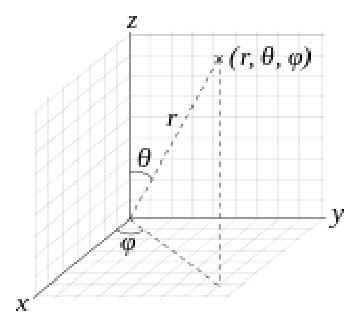
\includegraphics{157px-3D_Spherical.eps} \footnote{\ }

& 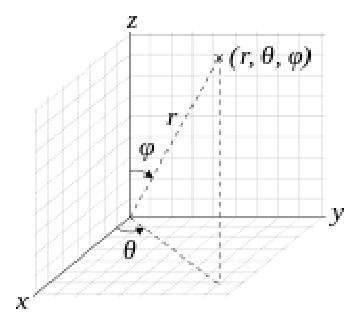
\includegraphics{157px-3D_Spherical_2.eps} \footnote{\ }
\end{tabular}
\end{center}



1-\small{`3D Spherical 2' by Dmcq - Own work. Licensed under Creative Commons Attribution-Share Alike 3.0 via Wikimedia Commons - \href{http://commons.wikimedia.org/wiki/File:3D_Spherical_2.svg\#mediaviewer/File:3D_Spherical_2.svg}{Wikipedia File} } 
\vskip0.1in
2- \small{`3D Spherical' by Andeggs - Own work. Licensed under Public domain via Wikimedia Commons - \href{http://commons.wikimedia.org/wiki/File:3D_Spherical.svg\#mediaviewer/File:3D_Spherical.svg}{Wikipedia File} }
}

\hrule
\vskip0.1in

\begin{problem} 
\marginpar{
	\thomasee{See page 893.} 
	\stewarts{See pages 827-833} 
	\larsonfive{See Larson 11.7.}
	}%
Let $P=(x,y,z)$ be a point in space. This point lies on a cylinder of radius $r$, where the cylinder has the $z$ axis as its axis of symmetry.  The height of the point is $z$ units up from the $xy$ plane. The point casts a shadow in the $xy$ plane at $Q=(x,y,0)$.  The angle between the ray $\vec{OQ}$ and the $x$-axis is $\theta$. Construct a graph in 3D of this information, and use it to develop the equations for cylindrical coordinates given above.
\end{problem}

\begin{problem}\label{derive spherical coordinates} Let 
\marginpar{
	\thomasee{See page 897.}
	\larsonfive{See Larson 11.7.}
	}% 
  $P=(x,y,z)$ be a point in space. This point lies on a sphere of
  radius $\rho$ (``rho''), where the sphere's center is at the origin
  $O=(0,0,0)$. The point casts a shadow in the $xy$ plane at
  $Q=(x,y,0)$.  The angle between the ray $\vec{OQ}$ and the $x$-axis
  is $\theta$, and is called the azimuth angle. The angle between
  the ray $\vec{OP}$ and the $z$ axis is $\phi$ (``phi''), and is
  called the inclination angle, polar angle, or zenith angle.  Construct
  a graph in 3D of this information, and use it to develop the
  equations for spherical coordinates given above.
\end{problem}

\marginpar{See the
  \href{http://en.wikipedia.org/wiki/Spherical_coordinate_system}{Wikipedia}
  or
  \href{http://mathworld.wolfram.com/SphericalCoordinates.html}{MathWorld}
  for a discussion of conventions in different disciplines.}%
	
There is some disagreement between different fields about the notation
for spherical coordinates.  In some fields (like physics), $\phi$
represents the azimuth angle and $\theta$ represents the inclination
angle.  In some fields, like geography, instead of the inclination angle, the
\emph{elevation} angle is given---the angle from the $xy$-plane (lines
of lattitude are from the elevation angle).
Additionally, sometimes the coordinates are written in a different
order.  You should always check the notation for spherical coordinates
before communicating using them.
\vskip0.1in
\hrule
\vskip0.1in
\noindent \Large After Class: \normalsize

\begin{problem}
For each curve below, set up an integral formula which would give the length, and sketch the curve. Do not worry about integrating them.  \marginpar{The reason I don't want you to actually compute the integrals is that they will get ugly really fast. Try doing one in Wolfram Alpha and see what the computer gives.}
\begin{enumerate}
\item The parabola $\vec p(t) = (t,t^2)$ for $t\in[0,3]$.
\item The ellipse $\vec e(t) = (4\cos t,5\sin t)$ for $t\in[0,2\pi]$.
\item The hyperbola $\vec h(t) = (\tan t,\sec t)$ for $t\in[-\pi/ 4,\pi/4]$.
\end{enumerate}
\end{problem}
To actually compute the integrals above and find the lengths, we would use a numerical technique to approximate the integral (something akin to adding up the areas of lots and lots of rectangles as you did in first semester calculus).

\valpo{
\begin{problem}
If you have never worked in Maple, you will want to spend some time familiarizing yourself with the program before our Lab day (keep reading if you are!). The link here takes you to a set of modules which will review several of the vector concepts we learned last week, but also introduce you to Maple. The Vector exploration contains a very nice visual on vector projections, which you should look at even if you are comfortable in Maple.
\vskip0.1in
The Connected Curriculum Project:\\
\href{https://www.math.duke.edu/education/ccp/resources/learn/index.html}{Introduction to Modules}
\vskip0.1in
\href{https://www.math.duke.edu/education/ccp/materials/mvcalc/javamaptutor/contents.html}{Maple Tutorial}
\vskip0.1in
\href{https://www.math.duke.edu/education/ccp/materials/mvcalc/vectors/index.html}{Vectors Exploration}
\end{problem}
}


%%% Local Variables: 
%%% mode: latex
%%% TeX-master: "215-problems"
%%% End: 


\chapter{Functions}
\minitoc \mtcskip
\input{05-Functions_ks_v2}
%\wrapup
%
%
%
\chapter{Derivatives}
%\note{Having them come up with how to generalize differential notation to higher dimensions, and then use differential notation as well, was too much. Perhaps I need one more problem right shortly after \ref{derive matrix derivative}.  In \ref{derive matrix derivative}, the students are taking differential notation and from it writing a matrix (it's how they discover the derivative).  What I need is to have the students write differential notation in terms of a matrix.  Perhaps this would be best after the next problem.  We're already finished with derivatives, so I'll put a note to myself to polish this up next semester. See my notes at the end as well.\\(From Jason) I added a pretty extensive problem having them practice differential notation.  We'll see if that helps them to get familiar with the ideas before moving to matrix multiplication.}


%There's a link in this file to dropbox.  Rather than have to hunt for it later, here it is.
\newcommand{\derivativehomeworklink}[1]{\href{http://db.tt/cSeKG8XO}{#1}}%
%
%
\noindent 
This unit covers the following ideas. In preparation for the quiz and exam, make sure you have a lesson plan containing examples that explain and illustrate the following concepts.  
\begin{enumerate}
\item Find limits, and be able to explain when a function does not have a limit by considering different approaches.
\item Compute partial derivatives. Explain how to obtain the total derivative from the partial derivatives (using a matrix).
\item Find equations of tangent lines and tangent planes to surfaces. We'll do this three ways.
\item Find derivatives of composite functions, using the chain rule (matrix multiplication).
\end{enumerate}
You'll have a chance to teach your examples to your peers prior to the exam.





\section{Limits}
In the previous chapter, we learned how to describe lots of different functions. In first-semester calculus, after reviewing functions, you learned how to compute limits of functions, and then used those ideas to develop the derivative of a function. The exact same process is used to develop calculus in high dimensions. One glitch that will prevent us from developing calculus this way in high dimensions is the epsilon-delta definition of a limit.  We'll review it briefly.  Those of you who want to pursue further mathematical study will spend much more time on this topic in future courses. 

In first-semester calculus, you learned how to compute limits of functions. Here's the formal epsilon-delta definition of a limit. 
\begin{definition}
 Let $f:\R\to\R$ be a function.
 We write $\ds \lim_{x\to c} f(x)=L$ if and only if for every $\epsilon>0$, there exists a $\delta>0$ such that $0<|x-c|<\delta$ implies $|f(x)-L|<\epsilon$.
\end{definition}
 We're looking at this formal definition here because we can compare it with the formal definition of limits in higher dimensions. The only difference is that we just put vector symbols above the input $x$ and the output $f(x)$.
\begin{definition}
 Let $\vec f:\R^n\to\R^m$ be a function.
 We write $\ds \lim_{\vec x\to \vec c} \vec f(\vec x)=\vec L$ if and only if for every $\epsilon>0$, there exists a $\delta>0$ such that $0<|\vec x-\vec c|<\delta$ implies $|\vec f(\vec x)-\vec L|<\epsilon$.
\end{definition}
We'll find that throughout this course, the key difference between first-semester calculus and multivariate calculus is that we replace the input $x$ and output $y$ of functions with the vectors $\vec x$ and $\vec y$. 
 
\begin{problem}
 For the function $f(x,y)=z$, we can write $f$ in the vector notation $\vec y=\vec f(\vec x)$ if we let $\vec x=(x,y)$ and $\vec y=(z)$. Notice that $\vec x$ is a vector of inputs, and $\vec y$ is a vector of outputs. 
 For each of the functions below, state what $\vec x$ and $\vec y$ should be so that the function can be written in the form $\vec y = \vec f (\vec x)$. \marginpar{The point to this problem is to help you learn to recognize the dimensions of the domain and codomain of the function.  If we write $\vec f:\R^n\to \R^m$, then $\vec x$ is a vector in $\R^n$ with $n$ components, and $\vec y$ is a vector in $\R^m$ with $m$ components.}  
\begin{enumerate}
 \item $f(x,y,z)=w$
 \item $\vec r(t)=(x,y,z)$
 \item $\vec r(u,v)=(x,y,z)$
 \item $\vec F(x,y)=(M,N)$
 \item $\vec F(\rho,\phi,\theta)=(x,y,z)$
\end{enumerate}
\end{problem}


You learned to work with limits in first-semester calculus without needing the formal definitions above. Many of those techniques apply in higher dimensions. 
The following problem has you review some of these technique, and apply them in higher dimensions.
\begin{problem}\marginpar{\bmw{See 14.2: 1-30 for more practice.}}%
 Do these problems without using L'Hopital's rule.
%, as there is not a good substitute for L'Hopital's rule in higher dimensions. \note{check this.}
\begin{enumerate}
 \item Compute $\ds \lim_{x\to 2} x^2-3x+5$ and then $\ds\lim_{(x,y)\to (2,1)} 9-x^2-y^2$.
 \item Compute $\ds\lim_{x\to 3}\frac{x^2-9}{x-3}$ and then $\ds\lim_{(x,y)\to (4,4)} \frac{x-y}{x^2-y^2}$.
 \item Explain why $\ds\lim_{x\to 0}\frac{x}{|x|}$ does not exist. [Hint: graph the function.]
\end{enumerate}
\end{problem}



In first semester calculus, we can show that a limit does or does not exist by considering what happens from the left, and comparing it to what happens on the right.  You probably used the following theorem extensively. 
\begin{quote}
 If $y=f(x)$ is a function defined on some open interval containing $c$, then $\ds\lim_{x\to c}f(x)$ exists if and only if  $\ds\lim_{x\to c^-}f(x) = \ds\lim_{x\to c^+}f(x)$.
\end{quote}
 A limit exists precisely when the limits from every direction exists, and all directional limits are equal. In first-semester calculus, this required that you check two directions (left and right). This theorem generalizes to higher dimensions, but it becomes much more difficult to apply. 

\begin{example}
 Consider the function $\ds f(x,y)=\frac{x^2-y^2}{x^2+y^2}$.
Our goal is to determine if the function has a limit at the origin $(0,0)$. We can approach the origin along many different lines.

One line through the origin is the line $y=2x$. If we stay on this line, then we can replace each $y$ with $2x$ and then compute
$$\ds\lim_{\text{\footnotesize $\begin{array}{c}(x,y)\to(0,0)\\ y=2x\end{array}$}}\frac{x^2-y^2}{x^2+y^2} 
= \lim_{x\to 0} \frac{x^2-(2x)^2}{x^2+(2x)^2}
= \lim_{x\to 0} \frac{-3x^2}{5x^2}
= \lim_{x\to 0} \frac{-3}{5}
=\frac{-3}{5}.$$
This means that if we approach the origin along the line $y=2x$, we will have a height of $-3/5$ when we arrive at the origin.
\end{example}
If the function $\ds f(x,y)=\frac{x^2-y^2}{x^2+y^2}$ has a limit at the origin, the previous problem suggests that limit will be $-3/5$.
\begin{problem}
 Please read the previous example. Recall that we are looking for the limit of the function $\ds f(x,y)=\frac{x^2-y^2}{x^2+y^2}$ at the origin (0,0). 
\marginpar{You may want to look at a graph in 
\href{https://sagecell.sagemath.org/?z=eJxL06jQqdS01aiIM9KtjDPS1AextEEsXq7k_LyS_NKi-IKc_BKNNB2gSl1jHWNNHY1KKCM5Pye_KCmxyDakqDRVJzk3scBWPSu1RF1Trzgjv1wDaARIq3EKNs2aALkvIzE=}{Sage} or \href{http://wolfr.am/ioCqzX}{Wolfram Alpha} (try using the ``contour lines'' option). %http://www.wolframalpha.com/input/?i=plot+%28x%5E2-y%5E2%29%2F%28x%5E2%2By%5E2%29
 As you compute each limit, make sure you understand what that limit means in the graph.}
Our goal is to determine if the function has a limit at the origin $(0,0)$.
\begin{enumerate}
 \item In the $xy$-plane, how many lines pass through the origin $(0,0)$? Give an equation a line other than $y=2x$ that passes through the origin.  Then compute $$\ds\lim_{\text{\footnotesize $\begin{array}{c}(x,y)\to(0,0)\\ \text{your line}\end{array}$}}\frac{x^2-y^2}{x^2+y^2}
= \lim_{x\to 0} \frac{x^2-(?)^2}{x^2+(?)^2}=\ldots.$$
 \item Give another equation a line that passes through the origin.  Then compute $$\ds\lim_{\text{\footnotesize $\begin{array}{c}(x,y)\to(0,0)\\ \text{your line}\end{array}$}}\frac{x^2-y^2}{x^2+y^2}.$$
 \item Does this function have a limit at $(0,0)$? Explain. \marginpar{\bmw{See 14.2: 41-50 for more practice.}\larsonfive{See Larson 13.2:23--36 and example 4 for more practice.}}%
\end{enumerate}
\end{problem}


The theorem from first-semester calculus generalizes as follows.
\begin{quote}
 If $\vec y=\vec f(\vec x)$ is a function defined on some open region containing $\vec c$, then $\ds\lim_{\vec x\to \vec c}\vec f(\vec x)$ exists if and only if the limit exists along every possible approach to $\vec c$ and all these limits are equal.
\end{quote}
There's a fundamental problem with using this theorem to check if a limit exists. Once the domain is 2-dimensional or higher, there are infinitely many ways to approach a point. There is no longer just a left and right side. To prove a limit exists, you must check infinitely many cases---that takes a \emph{really} long time.  The real power to this theorem is it allows to show that a limit does not exist.  All we have to do is find two approaches with different limits.



\begin{problem}
\marginpar{See \href{https://sagecell.sagemath.org/?z=eJyVVF1r2zAUfc-vuKQFy7PS2QndoCBY2dtgMFjfShtubLnW6lhCUlqrv37XlvOxtdtYEoKlc3TOufcKn50BfNFNBzcWn5Tj8FU5N_yMUfBZt618kBy-G6u6B1jmRTGbPaFlSc9Dks4-qc5Li6WfVbKGNauF6szOrze6Z7SDu9YL1r8L6XvW3y-zcL9MUz6D8WP8W-Sc5ymHFjeyFfNvmvSv4JyRWyrO5xyeVeUbUeQHFTTGaiyb4g2xRX9Qup5oUJBc-LvU8g0pSv9aa_laa5JKr8aHPuchF8aPi6GFHhq_bVlyDW5naywl7eoNbtoADTpAaNVWeUAPviFsKB9UPSysBOWg0wTS2aqSHZQNdg-0TU-61TayLpJ0MIv2diDQAHifLwr6y4oYMExAoHgEhAOwTyVIsvN6Z9em1Z7VPErx6SQvt2hE8kP6hI_eG7Tixu4IiMecuJx6MRa0jpWIWBFjY1_SeFQkVlYJd-pFilXOX7StpBWreLqmsnCokB3mzI9zmrp8EjwTamtaVQ6WQ_CwwH30ffLouWmxfEymohv9zE5yZpNYRLGXTqC1xGFR6ra44-M13a-XcZ1mEy2fzEYi3ebjxsA85eV8UURCzov0aJgJL3u_qti8p9t19Mkuislqj4f5r_oj4wR_me_lCZkcjBiaQ2j9W3NAG6TeBZFffOADJzbEiY-XFJpy_d9QTCYMWtxKb1UZB0J3EXnNgkB6EcDhVm1VJ449ozX24tgy36jysZPOidUf52f-qYLOyNKvLXqlxW3B6XuXzn4C8NyNiQ}{Sage}.}%
\marginpar{\bmw{See 14.2: 41-50 for more practice.}\larsonfive{See Larson 13.2:9--36 for more practice.}}%
 Consider the function $\ds f(x,y) = \frac{xy}{x^2+y^2}$.  Does this function have a limit at $(0,0)$?  

 \begin{enumerate}
 \item Examine the function at $(0,0)$ by considering the limit as you approach the origin along several lines. 
 \item Convert $\frac{xy}{x^2+y^2}$ to polar coordinates (i.e., a function of $r$ and $\theta$).  As $(x,y)$ approaches the origin, what does $r$ approach?  Take the limit of your polar coordinate function as $r$ approaches that value and interpret your result.
 \end{enumerate}
\end{problem}
\instructor{Try changing the above problem to polar coordinates and taking the limit as $r$ approaches 0.  Then try $\frac{x^2y}{x^2+y^2}$}

In all the examples above, we considered approaching a point by traveling along a line.  However, even if a function has a consistent limit along every line, that is not enough to always guarantee the function has a limit.  The theorem requires every approach be consistent, which includes parabolic approaches, spiraling approaches, and more.  Sometimes the straight-line paths happen to be consistent with each other, but a different path gives a different limit.  Give some thought to this in the optional challenge problem below.

\begin{problem*}[Challenge]\instructor{\href{https://sagecell.sagemath.org/?z=eJyVVNFq2zAUfQ_kH0RasDwrmZ2sGxQEK3sbDAbtW2nDjS3HWh1LSEpr9et3bdl1tnaUJSGxdI_OOfdckbMzQr6rqiE3Bh6lZeSHtLb7aC3JN1XXYi8YudZGNnuyTrNsPpvPHsHQqGU-iuezr7JxwkDu5rNClGRLSy4bfXTbnWop7sCxdpy29-sPPv6Iv58Sf7-OYzafkf6l3Vv4lKUxIzXsRM0XPxVqXJJzipIxP18w8iQLV_EsnWhAa6Mgr7I32JbtC9XVACMZ8vl3uNZvcGEjr8nWr8lGrvgyPLUp8ynXLqy6OB2p3KGm0RWxR1NCLnBX7WBXe1KBJUBqeZCOgCOuwlqXAZFltzCCSEsahUU8WxSiIXkFzR638UnVygTUKoo7scGA6RA4Cdamywy_kmww6YeKR4dY8VNlNMaRtXHqaLa6Vo6WLJCx4SjLD6B59Eu4iPXyOzD8xhyxEI5ZfjEm0je1Dd3w0BWlfThxOMsjI4qIWfks-CZlz8oUwvDNcLzE3qBrk74MnE3zGsM-8Z5wedC1zDvRzrtfwuh-NB9UdzXkD9HYeKWe6InVZGAbytAKy8EYBNFAdpvdsf7Ojut1WMfJAEsHuR6IV3va6JCnuJQtswBIWRafKCbcidZtCrpo8aZNQskqG7TGul_8KdAjTurPi5EfK6OE5l1AWC7_CogoDZif5-nqM-swIRPLv1ygbTT2v6PRCddg4CCckXkYC15LYCX1HPCvgbxcr4Ns-JQbrqHlU2yukvlDI6zlm39PUb9LA1aL3G0NOKn4bcbwfYcMvwGmS49T}{Sage}}
 Give an example of a function $f(x,y)$ so that the limit at $(0,0)$ along every straight line $y=mx$ exists and equals 0.  However, show that the function has no limit at $(0,0)$ by considering an approach that is not a straight line.
\end{problem*}


\section{Partial Derivatives}

Recall from first-semester calculus the following definition of the derivative.
\begin{dfn}
We define the derivative of a function $f$ at $x$ to be the limit
$$f'(x)=\frac{d}{dx}[f(x)]=\lim_{h\to 0}\frac{f(x+h)-f(x)}{h},$$
provided the limit exists. Whether you write $f'$ or $\frac{df}{dx}$ does not matter, as they both represent the same thing.  The notation $\frac{df}{dx}$ leads to the differential notation $dy=f'dx$, which we will use to generalize the derivative to all dimensions.
\end{dfn}
Before discussing the derivative of a function in higher dimensions, we first define partial derivatives. A matrix of partial derivatives will make up the total derivative.
\begin{dfn}[Partial Derivative]
 Let $f$ be a function.  The partial derivative of $f$ with respect to $x$ is the regular derivative of $f$, provided we hold all input variables constant except $x$.  If $f=f(x,y,z)$, we write any of 
 $$\frac{\partial f}{\partial x}=\frac{\partial}{\partial x}[f]=f_x = D_x f=\lim_{h\to 0}\frac{f(x+h,y,z)-f(x,y,z)}{h}$$
to mean the partial of $f$ with resepect to $x$.
 The partial of $f$ with respect to $y$, written $\ds \frac{\partial f}{\partial y}=f_y$, is the regular derivative of $f$, provided we hold all input variables constant except $y$. A similar definition holds for partials with respect to any variable.
\end{dfn}

\begin{problem}\marginpar{\bmw{See 14.3: 1-40 for more practice.}\larsonfive{See Larson 13.3:9--40 for more practice.} I strongly suggest you practice a lot of this type of problem until you can compute partial derivatives with ease.}%
 Find the indicated partial derivatives.
\begin{enumerate}
 \item For $f(x,y)=x^2+2xy+3y^2$ find $\ds\frac{\partial f}{\partial x}$ and $f_y$.
 \item For $f(x,y,z)=x^2y^3z^4$, find $f_x$, $\ds\frac{\partial f}{\partial y}$ and $D_z f$.
 \item For $\vec r(u,v) = (u,v,v\cos(uv))$, find $\ds\frac{\partial \vec r}{\partial u}$ and $\ds\frac{\partial \vec r}{\partial v}$.
 \item For $\vec F(x,y) = (-y,xe^{3y})$, find $\ds\frac{\partial \vec F}{\partial x}$ and $\ds\frac{\partial \vec F}{\partial y}$.
\end{enumerate}
\end{problem}

Since a partial derivative is a function, you can take partial derivatives of that function as well.  If you want to first compute a partial with respect to $x$, and then with respect to $y$, you would write $$f_{xy}=\ds\frac{\partial}{\partial y}\frac{\partial}{\partial x}f = \frac{\partial}{\partial y}\frac{\partial f}{\partial x} = \frac{\partial^2 f}{\partial y \partial x}.$$
The shorthand notation $f_{xy}$ is easiest to write, but in upper-level courses, we will use subscripts to mean other things. At that point, we'll use the fractional partial notation to avoid confusion.

\begin{problem}\label{second partials agree}\larsonfive{\marginpar{See Larson 13.3:71--80 for more practice.}}%
Consider the function $f(x,y)=3xy^3+e^{x^2}.$
\begin{enumerate}
 \item Compute the second partials $\ds \frac{\partial^2 f}{ \partial x^2}$, $\ds\frac{\partial^2 f}{\partial y \partial x}$, $\ds\frac{\partial^2 f}{\partial y^2}$, and $\ds\frac{\partial^2 f}{\partial x \partial y}$.
 \item For $f(x,y)=x^2+2xy+y^3$, compute both $f_{xy}$ and $f_{yx}$.  
 \item Make a conjecture about a relationship between $f_{xy}$ and $f_{yx}$.
 \item Use your conjecture to quickly compute $f_{xy}$ if $$f(x,y)=\tan^{2}(\cos(x)) (x^{49}+x)^{1000}+3xy.$$ 
\end{enumerate}
\end{problem}



The next problem will help you visualize what a partial derivative means in the graph of a surface.
\begin{problem} \label{cake introduction}\marginpar{See \href{https://sagecell.sagemath.org/?z=eJxtjUEOgjAQRfecoiEktHEwWOLCxazdewAMgSKNQJu2idTT26IxatxMZjL_vd_TBTzDQ7HUvPA1TzTqUbmqoz2EV1FBxYD610KUblrpPJbbPUv0BrWSs6OUww76OBmDVo3KYG5El4OVd4G8fEYb00zCGdmeYwMN9gh5jBB5d5FP3g2yvc7CWqz-Ozj44FiQrw7_47gYIeYcyJcmGdw00vQkOiItyUJ_BuQYk-sdXFnKEjuoG9XsARLFVGs}{Sage}.}%
\larsonfive{\marginpar{See Larson 13.3:53--58 for more practice.}}%
 Consider the function $f(x,y)=9-x^2-y^2$.  Construct a 3D surface plot of $f$ (see problem \ref{surface graph for a function of two variables}). We'll focus on the point $(2,1)$.
\begin{enumerate}
 \item Let $y=1$ and construct a graph in the $xz$ plane of the curve $z=f(x,1)=9-x^2-1^2$. Find an equation of the tangent line to this curve at $x=2$. Write the equation in the form $(z-z_0)=m(x-x_0)$.
 \item Let $x=2$ and construct a graph in the $yz$ plane of the curve $z=f(2,y)=9-2^2-y^2$. Find an equation of the tangent line to this curve at $y=1$. Write the equation in the form $(z-z_0)=m(y-y_0)$.
 \item Compute $f_x$ and $f_y$ and then evaluate each at $(2,1)$.  What does this have to do with the previous two parts?
 \item (We'll answer the remaining parts of this problem in class together.  If you complete them, we'll let you share with us your answer.) If the slope of a line $y=mx+b$ is $m$, then we know that an increase of $1$ unit in the $x$ direction will increase $y$ by $m$ units. Fill in the blanks, as they relate to the function $f(x,y)=9-x^2-y^2$ and the lines above.
\begin{itemize}
 \item Increasing $x$ by 1 unit when $y$ does not change will cause $z$ to increase by about \blank{1cm} units.
 \item Increasing $y$ by 1 unit when $x$ does not change will cause $z$ to increase by about \blank{1cm} units.
\end{itemize}
\item In the previous part, we said that $z$ increased by \emph{about} a certain amount.  Why did we not say that $z$ increases by \emph{exactly} that amount?
\end{enumerate}
\end{problem}

Once we have partial derivatives, we can calculate tangent lines to a surface. This means we can also find normal vectors and tangent planes as well.  Normal vectors to surfaces (i.e., vectors that are perpendicular to the surface) are extremely important in many areas, including physics, optics, and computer graphics.
\begin{problem} \label{cake plane introduction}\marginpar{See \href{https://sagecell.sagemath.org/?z=eJx9kUtvAiEYRff8CqImA8qYkUkTu2DdfbdNbSYMKOkIBFCH_voCPprax2YyX_Jx7uUg0UgiZo_1uKF13FBgA0OUrIjMX4wBmMqD5kEZDTvdQ2uUDsAyO5jQ9kiSdL5uSYsJipcfaGzHVYisWT5gYBesnEE2EMjNYByrnOgrAr36EIw2OQLygzsKX5Y71-1FcIq_5QyU-LlMZKkMgbe0b6iwU_xdC-9Zi-EUpt1fSZTERBoZLaR4R9o6IXSqdQdL67ngUfBgnAdyZHLZK5k4GMh4HeL5ojnmvIleVqQhciwWXzHxoXOBZQdf_PUtO4phMKfqJ6TJl49XCPyfYlynt6LKQu3QafGHznitNUdjTfHiwp-jWK_SdH73oropfpKp5u5d1yljF_YDmjyLHioPZ8n5jMCn7LDMSdtsgoHfmROy-BN9Vrcb}{Sage}.}%
  \marginpar{\bmw{See 14.6: 9-12 for more practice.}\larsonfive{See Larson 13.7:17--30 for more practice.}}%
 Consider the function $f(x,y)=9-x^2-y^2$ at the point $(2,1)$. From the previous problem, we know that increasing $x$ by 1 unit when $y$ does not change will cause $z$ to increase by about $f_x$ units. In terms of vectors, we have $(\Delta x, \Delta y, \Delta z) = (1,0,f_x)$ is a tangent vector to the surface. 
\begin{enumerate}
 \item At the point $(2,1)$, find a tangent vector to the surface in the $x$ direction (so compute $f_x(2,1)$ and put it in the vector $(1,0,f_x)$). Then give a vector equation of the tangent line to $f$ in the $x$ direction.
 \item At the point $(2,1)$, find a tangent vector to the surface in the $y$ direction. 
Then give a vector equation of the tangent line to $f$ in the $y$ direction.
 \item Give an equation of the tangent plane to $f$ at $(2,1)$. [Hint: we've found equations of planes before---see problems \ref{plane equation 2 lines} and \ref{plane equation normal point}. The cross product will come in handy.]
\end{enumerate}
\end{problem}

This next problem will help you see how parametric functions can simplify the process of finding tangent vectors and planes.
\begin{problem}\marginpar{\bmw{See 16.5: 27-30 for more practice.}\larsonfive{See Larson 15.5:35--38 for more practice.}}%
 Again, consider the function $f(x,y)=9-x^2-y^2$ at the point $(2,1)$. A parametrization of this surface is $\vec r(x,y) = (x,y,9-x^2-y^2)$. We'll use the parametrization to find an equation for the tangent plane at $(2,1,4)$.
\begin{enumerate}
 \item Compute $\ds\frac{\partial \vec r}{\partial x}(2,1)$. Then give a vector equation of the tangent line to $f$ in the $x$ direction.
 \item Compute $\ds\frac{\partial \vec r}{\partial y}(2,1)$. Then give a vector equation of the tangent line to $f$ in the $y$ direction.
 \item Give an equation of the tangent plane to $f$ at $(2,1)$. [Hint: See problem \ref{plane equation 2 lines}.]
\end{enumerate}
\end{problem}

\begin{problem}\marginpar{See \href{https://sagecell.sagemath.org/?z=eJx9kk-PwiAQxe_9FERNCu1oWusmXjjvfa8bNaQFJVsLAdSyn36havefuycCmfm9N28QuAdPaL9d5qusz3zut8tEO4ormJcghoOQJJmKU1c7qTrEugZpJTuXaDqcWDtAtWqVoanhTQrIyndOlwVJdE51q1zVYAFBqIAVAexhXkFJACnNauk8LRZPUQHVJ3Pmdmhihh25M7LexX4cegc3nkY3gO6sb7LuIOu3jltLK4KmKNY-ZFXgA6oPVZE0urmh9obzLszwgxbKo8Uzr50yNhE9FYtGisAhifD3ix9HxtdK_FoGp6K_5rghYB0zjsbEPgXWo7jnbasu6W9KAWF8P1LQ_xhlWLfnaQxVt6zjf0TqR2MZ7ucVye8KGfZ5Ga637X_J-9Hy1nCT1Sej20H24I4tnrzwBkmLZnETM0DPMdnhIYQ5m5DEHtQFa0DM6jDmzrDwv2gIrIRFuSEf2ELG4w}{Sage}.}%
\marginpar{\bmw{See 14.6: 9-12 for more practice.}\larsonfive{See Larson 13.7:17--30 for more practice.}}%
 Let $f(x,y)=x^2+4xy+y^2$.  Give two vector equations of tangent lines to the surface at $(3,-1)$. Then give an equation of the tangent plane.
\end{problem}

The next problem helps you generalize what you did above to construct the general formula for the tangent plane and normal vector to a surface $z=f(x,y)$ at the point $(a,b)$.

\begin{problem}\label{general tangent plane with partials}\marginpar{\bmw{Page 811 has the answer, but written in a slightly different form than you will get. In addition, they arrive at the solution in a completely different way.} }%%
\bmw{Recall that an equation of the tangent line to $y=f(x)$ at $x=c$ is $y-f(c)=f'(c)(x-c)$.\note{From Jason: I would rather that they make this connection later when they can just put vector symbols  I would rather that they make this connection only in problem \ref{tangent plane using matrix}, where it is much more natural.}}
Let $z=f(x,y)$ be a function whose partial derivatives exist.
\begin{enumerate}
\item Give two vectors tangent to the surface at $(x,y)=(a,b)$.
\item Give a normal vector to the surface at $(a,b)$.
\item Give an equation of the tangent plane to the surface at $(a,b)$.
\end{enumerate}
\end{problem}

The next problem generalizes the tangent plane and normal vector calculations above to work for a parametric surface $\vec r(u,v)$.\note{Should this problem and the previous problem be swapped?  Think about it...}
\begin{problem}\marginpar{See \href{https://sagecell.sagemath.org/?z=eJx9kM1uwjAQhO95ihUgxQ4uhbSVevG5954rVZZjwMLY1voH0aevEwhEFerJu9buN7ODJLFMOUmNdIFkyiA1QdtLRSsfudEhEiQt8_q5pbSq5ttkZdTOgrAdeKdtrDwfXuIjA-mMQ16j6moGQf8o3q4Lacm9QHFUEbX89sYVKIOivmavRYvkUkDbeF0a54XU8czXq7deD2TCrMJDBMl88DVBTfXjXsuDVSHwFwpzuAw_BiXejj6uNq6gHSplyyl_WGW-95aVjA5DhYnjqtPbLSmxYR6bfLl8kEhjiCxEgZH3Yd2h7zfBszLGnerJZr5twv-rDoXdqbpPzRth1aNTU3N3sszNFD5mWFJ42rANZVesT-jNgN3HoyGzT9WBDrDI_KvfXDD46EMa_kouixmtwt6diKe_OvC8aA}{Sage}.}%
\marginpar{\bmw{See 16.5: 27-30 for more practice.}\larsonfive{See Larson 15.5:35--38 for more practice.}}%
 Consider the cone parametrized by $\vec r(u,v)=(u\cos v, u\sin v,u)$.
 \begin{enumerate}
 \item Give vector equations of two tangent lines to the surface at $(2,\pi/2)$ (so $u=2$ and $v=\pi/2$).
 \item Give a normal vector to the surface at $(2,\pi/2)$.
 \item Give an equation of the tangent plane at $(2,\pi/2)$.
 \end{enumerate}
\end{problem}


\section{The Derivative}\label{sec:derivative}
\begin{remark}
 In problem \ref{cake introduction}, we learned the following for  $z=f(x,y)$.
\begin{itemize}
 \item Increasing $x$ by 1 unit when $y$ remains constant will cause $z$ to increase by about $f_x$ units.
 \item Increasing $y$ by 1 unit when $x$ remains constant will cause $z$ to increase by about $f_y$ units.
\end{itemize}
We will use these facts to introduce differential notation for functions of several variables, and then define the total derivative as a matrix of partial derivatives.
\end{remark}

\begin{problem}
 Fill in the blanks. For this example, consider the function $z=f(x,y)$.
\begin{itemize}
 \item Remember that increasing $x$ by 1 when $\Delta y=0$ will cause $z$ to increase by about $f_x$ units.  So increasing $x$ by only $\frac{1}{2}$ when $\Delta y=0$ will cause $z$ to increase by about \underline{$\frac{1}{2}f_x$}. In a similar fashion, increasing $y$ by $\frac{1}{10}$ when $\Delta x=0$ will cause $z$ to increase by about \blank{1cm}. Combining these two ideas, we find that if $\Delta x=\frac{1}{2}$ and $\Delta y=\frac{1}{10}$ then $\Delta z\approx$ \blank{2cm}. 
 \item Increasing $x$ by $dx$ when $\Delta y=0$ will cause $z$ to increase by about \blank{1cm}. Increasing $y$ by $dy$ when $\Delta x=0$ will cause $z$ to increase by about \blank{1cm}. So combining these two ideas, we find that if $\Delta x=dx$ and $\Delta y=dy$ then $\Delta z\approx$ \blank{2cm}. [Hint: read the definition below to see if you're on the right track.]
\end{itemize}
\end{problem}

Based on the answer from the previous problem, we define the following.
\begin{definition}
In first-semester calculus, if $y=f(x)$, we defined the differential of $f$ to be
$$df = f'\,dx=\frac{df}{dx}\,dx,$$ where $dx$ represents a change in $x$.
We can think of this as ``A tiny change in the output $f(x)$ is approximately the same as the derivative, multiplied by a small change in the input $x$.''

Based on the defintion from first semester calculus, and the answer from the previous problem, if $z=f(x,y)$ we'll define the differential of $f$ to be 
$$df= \frac{\partial f}{\partial x}dx+ \frac{\partial f}{\partial y}dy,$$
or in short-hand notation $df=f_xdx+f_ydy$, 
where $dx$ and $dy$ are independent variables which represent small changes in $x$ and $y$. 
\end{definition}

In the next problem, you will use differential notation to discover the derivative of a function in high dimensions.
We would like to be able to think of differential notation in all dimensions in the same way we think about it in one dimension. Ideally we could say ``A tiny change in the output $f(x,y)$ is approximately the same as the derivative $Df(x,y)$, multiplied by a small change in the inputs $x$ and $y$.''

\begin{problem}\label{derive matrix derivative}\marginpar{See Section~\ref{review matrices} to refresh on how to do matrix multiplication.}%
In each problem below, your job is to find a matrix $M$ so that the matrix product is the same as the corresponding differential notation. 
\begin{enumerate}
 \item  Let $f(x,y)=z$. Find a matrix $M$ so that 
$$df=f_xdx+f_ydy=M\begin{bmatrix}dx\\dy\end{bmatrix}.$$
 \item  Let $f(x,y,z)=w$. Find a matrix $M$ so that 
$$df=f_xdx+f_ydy+f_zdz=M\begin{bmatrix}dx\\dy\\dz\end{bmatrix}.$$
 \item  Let $\vec r(t)=(x,y)$. Find a matrix $M$ so that 
$$d\vec r=\frac{d\vec r}{dt}dt=\begin{pmatrix}\frac{dx}{dt}dt\\\frac{dy}{dt}dt \end{pmatrix}=Mdt.$$
 \item  Let $\vec r(u,v)=(x,y,z)$. We will think of $\dfrac{\partial \vec r}{\partial u}=\begin{bmatrix}x_u\\y_u\\z_u\end{bmatrix}$ and $\dfrac{\partial \vec r}{\partial v}=\begin{bmatrix}x_v\\y_v\\z_v\end{bmatrix}$ as column vectors (single-column matrices).  Find a matrix $M$ so that 
$$d\vec r=\frac{\partial \vec r}{\partial u}du+\frac{\partial \vec r}{\partial v}dv=M\begin{bmatrix}du\\dv\end{bmatrix}.$$
\end{enumerate}
\end{problem}



\begin{definition}\marginpar{The derivative of a function, $D\vec f$, is given many names in the literature.  It's called the total derivative, the matrix derivative, the Jacobian, the Jacobian matrix, and more. We'll just call $D\vec f$ the derivative.}
The derivative of a function $\vec f:\R^n\to \R^m$, where $\vec y=\vec f(\vec x)$, is a matrix, written $D\vec f$ and read ``the derivative of $f$''. The columns of the matrix are the partial derivatives of the function. The order in which you list the input variables of $f$ is precisely the order in which the partials occur in the columns of the matrix.

 This matrix $D\vec f$ gives the best possible linear approximation to changes in the outputs, based upon changes in the inputs. We write the previous sentence symbolically as $d\vec y = D\vec f d\vec x$. 
\end{definition}
In first-semester calculus, we wrote the derivative of $y=f(x)$ in differential notation as $dy=f'dx$.  To generalize, we put a vector above each variable and change $f'$ from a number (a one-by-one matrix) to a matrix. This results in the derivative of $\vec y=f(\vec x)$ being written in differential notation as $d\vec y = D\vec f d\vec x$.  This more general differential notation is valid in all dimensions.

Remember, to find the derivative of a function, compute all the partial derivatives and then place them in the columns of the matrix. Every input variable gets a column. {\it Every input variable gets a column. {\bf Every input variable gets a column.}} 

\begin{problem}
\marginpar{This \derivativehomeworklink{handwritten file} has 6 problems, together with solutions, that you can use as extra practice.}
 For each function below, state the dimensions of the domain and codomain (numbers of inputs and outputs) and write the function in the form $f:\R^n\to R^m$ (figure out what $n$ and $m$ are).  Then find the derivative (as a matrix). How does the number of rows and columns relate to $n$ and $m$? Remember, every input variable gets a column. \marginpar{I'll have 4 people present this one in class.}
\begin{enumerate}
 \item $f(x,y)=x^2+4xy+y^3$
 \item $f(x,y,z)=x^2-yz^3$
 \item $\vec r(t)=(\cos t, \sin t)$ (Remember to place vectors in columns.)
 \item $\vec r(t)=(\cos t, \sin t,t)$
 \item $\vec r(a,t)=(a\cos t, a\sin t,t)$
 \item $\vec T(r,\theta)=(r\cos \theta, r\sin \theta)$
 \item $\vec F(x,y)=(2x+3y,4x+5y)$
 \item $\vec F(x,y,z)=(2x+3y-5z,4x+5y+z^2, xyz)$
\end{enumerate}
\end{problem}

Once we have the multivariable (matrix) derivative, almost every idea from first-semester calculus can be generalized to all dimensions by just replacing $f'$ with $Df$ and putting vector symbols above the inputs and outputs. As a first example, let's examine how tangent lines generalize to tangent planes.

\begin{remark}
  In problem \ref{differentials give tangent lines}, we saw that the differential notation $dy=f'dx$ allowed us to write an equation of the tangent line to $y=f(x)=x^2$ at $x=3$. Here's a recap of what we did.
\begin{quote} The derivative is $f'(x)=2x$ which at $x=3$ equals $f'(3)= 6$. The graph of the function passes through the point $(3,f(3)) = (3,9)$. If $(x,y)$ is any point on the tangent line, then the change from $(3,9)$ to $(x,y)$ is given by $(dx,dy)=(x,y)-(3,9)=(x-3,y-9)$.  Differential notation then says $dy=f'(3)dx$, or in other words, $(y-9)=6(x-3)$.  
\end{quote}
Tangent lines pop out instantly from differential notation. Tangent planes will ``pop out'' too, as well as tangent objects in any dimension. 
\end{remark}


\begin{problem}\label{tangent plane using matrix}\marginpar{See \href{https://sagecell.sagemath.org/?z=eJx9kEFuwyAQRfecAqkLQzKOsKNK6YKTVE2FMDQoLiCgDfT0BTvuopW6Gc1IM-__-ZpkKJQ_9fk89uU8Ip84GWEA3SqlCD3oDyuTcRYLO2HvjE3Icz-7dJyIhnrfH-FIgZR7g50X0qTC2eGRIr_nyw3xCbB0swu8C2rqAEfzpfjImgT-VDK5EJHOXB8mozXJFOmyDWXlVE2ybpLnARjovJh8oRCTCIk3iXQx8mpVjPz0o1fUPLtb9xfC2qNlg-D_KS4I-6a65tfPwqqFJoJ4VykY-bqAW5qbrR3J_Uj3d_6OlH6o0xor4LrJlrRqbuxXbKeqES_uRjz9BkpQfFk}{Sage}.}%
Read the remark above. Then give an equation of the tangent plane to $f(x,y)=9-x^2-y^2$ at $(2,1)$ by using differential notation. Try doing so without using the steps below, but rather just mimic what we did in the remark above (replacing inputs and outputs with vectors, and the derivative with the appropriate matrix). If you need the following steps, then use them. Compare with problem \ref{cake plane introduction}.
\begin{enumerate}
 \item Find $Df(x,y)$ and then $Df(2,1)$. You should have two matrices. Also Find the point $(2,1,f(2,1))$ on the graph of the surface.
 \item If $(x,y,z)$ is any point on the tangent plane, find the change from $(2,1, f(2,1))$ to $(x,y,z)$ (subtract vectors).  This change is $(dx,dy,dz)$.
 \item We'll use differential notation to finish this problem. We want to generalize $dy=f'dx$ (a change in outputs equals the derivative times a change in inputs), so we will use the notation $d\vec y = D\vec fd\vec x$. Recall the following:
\begin{itemize} 
\item  The inputs to $z=f(x,y)$ are $x$ and $y$, so the input vector is $\vec x=(x,y)$.  The output is $z$, so the output vector is $\vec y= (z)$.
\item The change in inputs is $(dx,dy)$.  The change in outputs is $(dz)$. 
\item The differential notation $d\vec y=D\vec f\ d\vec x$ then, in this case, becomes $\begin{bmatrix}dz\end{bmatrix}=Df\begin{bmatrix}dx \\ dy\end{bmatrix}$. This means a very small change in the output $z$ equals the derivative times very small changes in the inputs $x$ and $y$.
\end{itemize}
Now use the differential notation $\begin{bmatrix}dz\end{bmatrix}=Df\begin{bmatrix}dx \\ dy\end{bmatrix}$ to write a matrix equation of the tangent plane (use $Df(2,1)$ from part 1 and $dx$, $dy$, and $dz$ from part 2). Then perform the matrix multiplication to get an equation of the tangent plane. Compare your answer with problem \ref{cake plane introduction}.
\end{enumerate}
\end{problem}

\begin{problem}
  Suppose $z=f(x,y)$ has a derivative $Df(x,y)$. Use differential notation to give an equation of the tangent plane to the surface at $(x,y)=(a,b)$ (use the steps from the previous problem if needed). Multiply out any matrix products. What is a normal vector to the plane? Compare with problem \ref{general tangent plane with partials}.
\end{problem}

\section{The Chain Rule}

Let's recall the chain rule from first-semester calculus. 

\begin{theorem}[The Chain Rule]
 Let $x$ be a real number and $f$ and $g$ be functions of a single real variable. Suppose $f$ is differentiable at $g(x)$ and $g$ is differentiable at $x$. The derivative of $f\circ g$ at $x$ is 
$$(f\circ g)'(x) = \frac{d}{dx}(f\circ g)(x) = f'(g(x))\cdot g'(x).$$
\end{theorem}

Some people remember the theorem above as ``the derivative of a composition is the derivative of the outside (evaluated at the inside) multiplied by the derivative of the inside.'' If $u=g(x)$, we sometimes write $\ds \frac{df}{dx}=\frac{df}{du}\frac{du}{dx}$. The following problem is designed to help you master the notation.

\begin{problem}\label{chain rule review problem}
 Suppose we know that $\ds f'(x) = \frac{\sin(x)}{2x^2+3}$ and $g(x)=\sqrt{x^2+1}$. Notice we don't know $f(x)$.  This is actually quite common in real life, as we can often measure how something changes (a derivative) without knowing the actual function.
\begin{enumerate}
 \item What is $f'(x)$ and $g'(x)$?
 \item What is the difference between $f'(x)$ and $f'(g(x))$? State $f'(g(x))$.
 \item Use the chain rule to compute $(f\circ g)'(x)$.
\end{enumerate}
\end{problem}

We now generalize to higher dimensions. If I want to write $\vec f(\vec g(\vec x))$, then $\vec x$ must be a vector in the domain of $g$.  After computing $\vec g(\vec x)$, we must get a vector that is in the domain of $f$. 

\begin{problem}\label{horse track chain rule introduction}
 Consider $f(x,y)=9-x^2-y^2$ and $\vec r(t)=(2\cos t, 3\sin t)$. For this problem, imagine the following scenario.  A horse is running around outside in the cold. The horse's position at time $t$ is given by the elliptical path $\vec r(t)$. The temperature of the air at any point $(x,y)$ is given by $T=f(x,y)$.  
\begin{enumerate}
 \item\label{item:1} At time $t=0$, what is the horse's position $\vec r(0)$, and what is the temperature $f(\vec r(0))$ at that position? Find the temperatures at $t=\pi/2$, $t=\pi$, and $t=3\pi/2$ as well. 
 \item In the plane, draw the path of the horse for $t\in [0,2\pi]$. Then, on the same 2D graph, include a contour plot of $f$. Make sure you include the level curves that pass through the points in part~\ref{item:1}. (See  \ref{parametric curve in plane example} and \ref{cake level curves plot} if you need help.) At the points addressed in part~\ref{item:1}, write the temperature on the curve.
 \item\marginpar{This idea will lead to a very important optimization technique, Lagrange multipliers, later in the semester.}%
 As the horse runs around, the temperature of the air around the horse is constantly changing. 
At which $t$ does the temperature around the horse reach a maximum?  A minimum?  Explain, using your graph. 
 \item\label{item:2} As the horse moves past the point at $t=\pi/4$, is the temperature of the surrounding air increasing or decreasing? Use your graph to explain.
 \item \instructor{See \href{https://sagecell.sagemath.org/?z=eJyFj0FuwjAQRfc-RXaMk0kV2WLBwrforoLKGEdYmNgaOyK5fU3oIqCq7N5i_pv_e5hw5mrXTgfRzgfBCDJXIGoTUiGsZJ3cUIgzFlX0IcsT9FhSrUTJEeZfqELUxuVZdR9bzmKjoiZ9tZmc-b7HwLuU4W7nzVcP9UJ7rCBjh6KOrihM8IHUhuxpg_nszGWwKSn5Vtf946meRCydww1iAROGHEZ6yP4atEiOmtQnjRa9PlqfFubNaxfC1Xc92cfdaoLAVSX-A1SMc_Q}{Sage}.}%
Draw the 3D surface plot of $f$. In the $xy$-plane of your 3D plot (so $z=0$) add the path of the horse. In class, we'll project the path of the horse up into the 3D surface (give it a try yourself first). 
\end{enumerate}
\end{problem}

\begin{problem}
 Consider $f(x,y)=9-x^2-y^2$ and $\vec r(t)=(2\cos t, 3\sin t)$, which means $x=2\cos t$ and $y=3\sin t$.
\begin{enumerate}
 \item\marginpar{Try to always remember the following summary of differential notation: a change in the outputs equals the derivative times a change in the inputs.}%
For the function $\vec r(t)=(x,y)$, the input is $t$ and the outputs are $x$ and $y$.  So differential notation  states that 
$$\begin{pmatrix}dx\\dy\end{pmatrix}=D\vec r(t)\begin{pmatrix}dt\end{pmatrix}.$$
 Compute $D\vec r(t)$.
 \item For the function $T=f(x,y)$, the inputs are $x$ and $y$, and the output is temperature $T$. Differential notation  states that 
$$\begin{pmatrix}dT\end{pmatrix}=Df(x,y)\begin{pmatrix}dx\\dy\end{pmatrix}.$$
 Compute $Df(x,y)$.
 \item Now we want to find out how the temperature $T$ changes with respect to time $t$. We already know 
 $$\begin{pmatrix}dx\\dy\end{pmatrix}=D\vec r(t)\begin{pmatrix}dt\end{pmatrix} \quad \text{and}\quad 
 \begin{pmatrix}dT\end{pmatrix}=Df(x,y)\begin{pmatrix}dx\\dy\end{pmatrix}.$$ 
 Use these two differential facts to write a change in temperature $dT$ in terms of a change in time $dt$. 
 \item Compute the matrix product $Df(x,y)D\vec r(t)$, and then substitute $x=2\cos t$ and $y=3\sin t$. You should have an expression of the form $dT = (?) dt$ where $?$ is some function of $t$.   
 \item What is $df/dt$ (i.e., $dT/dt$) at $t=\pi/4$? Is it positive or negative? Compare with part~\ref{item:2} of the previous problem.
\end{enumerate}
\end{problem}

\begin{problem}
 Consider $f(x,y)=9-x^2-y^2$ and $\vec r(t)=(2\cos t, 3\sin t)$.
\begin{enumerate}
 \item Writing $\vec r(t)=(2\cos t, 3\sin t)$ means $x=2\cos t$ and $y=3\sin t$. In $f(x,y)$, replace $x$ and $y$ with what they are in terms of $t$. This will give you $f$ as a function of $t$. 
 \item Construct a graph of $f(t)$ (use software to draw this if you like). From your graph, at what time values do the maxima and minima occur?
 \item Compute $df/dt$ (the derivative as you did in first-semester calculus).
 \item What is $df/dt$ at $t=\pi/4$?
 \item Compare your work with the previous problem.
\end{enumerate}
\end{problem}

The previous three problems all focused on exactly the same concept.  The first looked at the concept graphically, showing  what it means to write $(f\circ \vec r)(t)=f(\vec r(t))$. The second tackled the problem by considering matrix derivatives.  The third reduced the problem to first-semester calculus.  In all three cases, we wanted to understand the following problem.
\begin{quote}
 If $z=f(x,y)$ is a function of $x$ and $y$, and both $x$ and $y$ are functions of $t$, so in vector form we can write $\vec r(t)=(x(t),y(t))$, then find how quickly $f$ changes as you change $t$. In other words, what is the derivative of $f$ with respect to $t$. Notationally, we seek $\ds \frac{df}{dt}$ which formally is written $\ds \frac{d}{dt}[f(x(t),y(t))]$ or $\ds \frac{d}{dt} [f(\vec r(t))].$
\end{quote}
The second problem above gave us an example of the multivariable chain rule.
\begin{theorem}[The Chain Rule]\label{chain rule def}
 Let $\vec x$ be a vector and $\vec f$ and $\vec g$ be functions so that the composition $\vec f(\vec g(\vec x))$ makes sense (the output of $g$ can be used as an input to $f$). Suppose $\vec f$ is differentiable at $\vec g(\vec x)$ and $\vec g$ is differentiable at $\vec x$. The derivative of $\vec f\circ \vec g$ at $\vec x$ is 
$$D(\vec f\circ \vec g)(\vec x) = D\vec f(\vec g(\vec x))\cdot D\vec g(\vec x).$$
In other words, the derivative of a composition is equal to the derivative of the outside (evaluated at the inside), multiplied by the derivative of the inside. 
\end{theorem}
This is exactly the same as the chain rule in first-semester calculus.  The only difference is that now we have vectors above every variable and function, and we replaced the one-by-one matrices $f'$ and $g'$ with potentially larger matrices $Df$ and $Dg$. If everything is written in vector notation, the chain rule in any dimensions is the same as the chain rule in one dimension.

\begin{problem}\marginpar{\bmw{See 14.4: 1-6 for more practice.}\larsonfive{See Larson 13.5:1--6 for more practice (you can check answers in the back of the book).  Don't use the formulas on pages 925--930.  Instead, use matrix multiplication.  The formulas are just a way of writing matrix multiplication without writing down the matrices, and only work for functions from $\RR^n\to\RR$.  Our matrix multiplication method works for any function from $\RR^n\to\RR^m$.}}%
 Suppose $f(x,y) = x^2+xy$ and $x=2t+3$ and $y=3t^2+4$.
 \begin{enumerate}
  \item Rewrite the parametric equations $x=2t+3$ and $y=3t^2+4$ in vector form, so we can apply the chain rule. This means you need to create a function $\vec r(t) = (\blank{1in}, \blank{1in})$.
  \item Compute the derivatives $Df(x,y)$ and $D\vec r(t)$. 
  \item The chain rule states that $D(f\circ \vec r)(t) = Df(\vec r(t))D\vec r(t)$. What is the difference between $Df(x,y)$ and $Df(\vec r(t))$. [Hint: see problem \ref{chain rule review problem}.]
  \item Use the chain rule to compute $D(f\circ \vec r)(t)$. What is $df/dt$?
%  \item Now, without any matrix multiplication, replace $x$ and $y$ in $f=x^2+xy$ with what they are in terms of $t$, and then use first-semester calculus to find $df/dt$.
 \end{enumerate}
\end{problem}

\begin{problem}\marginpar{\bmw{See 14.4: 7-12 for more practice.}\larsonfive{See Larson 13.5:7--10 for more practice (remember to use matrix multiplication, not the formulas from the book).}}%
 Suppose $f(x,y,z) = x+2y+3z^2$ and $x=u+v$, $y=2u-3v$, and $z=uv$.  This means that changing $u$ and $v$ should cause $f$ to change. Our goal is to find $\partial f/\partial u$ and $\partial f/\partial v$. Try doing this problem without looking at the steps below, but instead try to follow the patterns in the previous problem on your own. 
 \begin{enumerate}
  \item Rewrite the equations for $x,y,$ and $z$ in vector form $\vec r(u,v)=(x,y,z)$. %If you were to graph $\vec r$, what kind of graph would you make?
  \item Compute $Df(x,y,z)$ and $D\vec r(u,v)$.  
  \item Use the chain rule (matrix multiplication) to find $D(f\circ \vec r)(u,v)$.  Notice that since this composite function has 2 inputs, namely $u$ and $v$, we should expect to get two columns when we are done.
  \item What are $\partial f/\partial u$ and $\partial f/\partial v$? [Hint: remember, each input variable gets a column.]
 \end{enumerate}
\end{problem}

\begin{problem}
 Suppose $\vec F(s,t) = (2s+t,3s-4t,t)$ and $s=3pq$ and $t=2p+q^2$.  This means that changing $p$ and $q$ should cause $\vec F$ to change. Our goal is to find $\partial \vec F/\partial p$ and $\partial \vec F/\partial q$. Note that since $\vec F$ is a vector-valued function, the two partial derivatives should be vectors. Try doing this problem without looking at the steps below, but instead try to follow the patterns in the previous problems on your own. 
 \begin{enumerate}
  \item\label{item:3} Rewrite the parametric equations for $s$ and $t$ in vector form.
  \item Compute $D\vec F(s,t)$ and the derivative of your vector function from part~\ref{item:3}.
  \item Use the chain rule (matrix multiplication) to find the derivative of $\vec F$ with respect to $p$ and $q$.  How many columns should we expect to have when we are done multiplying matrices?
  \item What are $\partial \vec F/\partial p$ and $\partial \vec F/\partial q$? 
 \end{enumerate}
\end{problem}

%\begin{problem}
% \note{Maybe move this problem down after a few of the general problems that emphasize the concepts above.}Suppose $\vec F(u,v) = (3u-v,u+2v,3v)$,  $\vec G(x,y,z)=(x^2+z, 4y-x)$, and $\vec r(t) = (t^3, 2t+1, 1-t)$.  We want to examine $\vec F(\vec G(\vec r(t))$.  This means that $\vec F\circ \vec G\circ \vec r$ is a function from $\RR^n\to\RR^m$ for what $n$ and $m$?  Similar to first-semester calculus, since we have two functions nested inside of each other, we'll just need to apply the chain rule twice.  Our goal is to find $d\vec F/dt$.  Try to do this problem without looking at the steps below.
% \begin{enumerate}
%  \item Compute $D\vec F(u,v)$, $D\vec G(x,y,z)$, and $D\vec r(t)$.
%  \item Use the chain rule (matrix multiplication) to find the derivative of $\vec F$ with respect to $t$.  What size of matrix should we expect for the derivative?
% \end{enumerate}
%\end{problem}



\begin{problem}\marginpar{\bmw{See 14.4: 13-24 for more practice.  Don't use the ``branch diagram'' in the book---use matrix multiplication instead. The branch diagram is just a way to express matrix multiplication without having to introduce matrices.}\larsonfive{See Larson 13.5:7--10 for more practice.}}%
 Suppose $w=f(x,y,z)$ and $x,y,z$ are all function of one variable $t$ (so $x=g(t), y=h(t), z=k(t)$).  
 Find a general formula for $dw/dt$ that involves partials of $f$ and derivatives of $x$, $y$, and $z$. Try doing this problem without looking at the steps below, but instead try to follow the patterns in the previous problems.
\begin{enumerate}
 \item Rewrite the parametric equations for $x$, $y$, and $z$ in vector form $\vec r(t) = (x,y,z)$.
 \item Compute $Dw(x,y,z)$ and $D\vec r(t)$. 
 \item Multiply the matrices together to get $D(w\circ r)(t)$.  The matrix should have one entry. State what $dw/dt$ equals.
\end{enumerate}
\end{problem}


\begin{problem}\larsonfive{\marginpar{See Larson 13.5:19--26 for more practice.}}%
 Suppose $z=f(s,t)$ and $s$ and $t$ are functions of $u$, $v$ and $w$.  Use the chain rule to give a general formula for $\partial z/\partial u$, $\partial z/\partial v$, and $\partial z/\partial w$. 
\end{problem}

You've now got the key ideas needed to use the chain rule in all dimensions. You'll find this shows up many places in upper-level math, physics, and engineering courses. The following problem will show you how you can use the general chain rule to get an extremely quick way to perform implicit differentiation from first-semester calculus.

\begin{problem}\marginpar{\bmw{See 14.4: 25-32 to practice using the formula you developed.}  To practice the idea developed in this problem, show that if $w=F(x,y,z)$ is held constant at $w=c$ and we assume that $z=f(x,y)$ depends on $x$ and $y$, then $\frac{\partial z}{\partial x} = -\frac{F_x}{F_z}$ and $\frac{\partial z}{\partial y} = -\frac{F_y}{F_z}$. \bmw{This is done on page 798 at the bottom. }}%
\larsonfive{\marginpar{See Larson 13.5:27--30 for more practice, and see pages 929--930 for how the book derives these formulas.}}%
 Suppose $z=f(x,y)$.  If $z$ is held constant, this produces a level curve. As an example, if $f(x,y) = x^2+3xy-y^3$ then $5=x^2+3xy-y^3$ is a level curve. Our goal in this problem is to find $dy/dx$ in terms of partial derivatives of $f$.
\begin{enumerate}
 \item Suppose $x=x$ and $y=y(x)$, so $y$ is a function of $x$.  We can write this in parametric form as $\vec r(x) = (x,y(x))$. We now have $z=f(x,y)$ and $\vec r(x)=(x,y(x))$.  Compute both $Df(x,y)$ and $D\vec r(x)$ symbolically.  Don't use the function $f(x,y)=x^2+3xy-y^3$ until the last step. 
 \item\label{item:4} Use the chain rule to compute $D(f(\vec r(x)))$. What is $dz/dx$ (i.e., $df/dx$)?
 \item Since $z$ is held constant, we know that $dz/dx=0$. Use this fact, together with part~\ref{item:4} to explain why $\ds \frac{dy}{dx} = -\frac{f_x}{f_y} = -\frac{\partial f/ \partial x}{\partial f/ \partial y}$.
 \item For the curve $5=x^2+3xy-y^3$, use this formula to compute $dy/dx$.
\end{enumerate}

\end{problem}

%%% Local Variables: 
%%% mode: latex
%%% TeX-master: "215-problems"
%%% End: 

\minitoc \mtcskip
\input{06-Derivatives-new_ks_v2}
%\wrapup
%
\chapter{Motion}
\vspace{-1.25cm}
\minitoc \mtcskip
\input{07-Motion_ks_v2}
%\wrapup
%
\chapter{Line Integrals}
\minitoc \mtcskip
\input{08-Line-Integrals_ks_v2}
%\wrapup
%
%
%
\chapter{Optimization}
\minitoc \mtcskip
\input{09-Optimization_ks_v2}
%\wrapup
%
%
\chapter{Double Integrals}
\minitoc \mtcskip
\input{10-Double-Integrals_ks_v2}
%\wrapup
%
%%\end{document}
%
%
\chapter{Surface Integrals}
\minitoc \mtcskip
\input{11-Surface-Integrals_ks_v2}
%\wrapup
%
\chapter{Triple Integrals}
\minitoc \mtcskip
\input{12-Triple-Integrals_ks_v2}
%\wrapup

\begin{comment}
\end{comment}
\end{document}
